\newpage
\appendix

% Renumber appendix figures and tables as A1, A2, ... and A1, A2, ...
\setcounter{figure}{0}
\setcounter{table}{0}
\renewcommand{\thefigure}{A\arabic{figure}}
\renewcommand{\thetable}{A\arabic{table}}

\section*{Appendix}
\addcontentsline{toc}{section}{Outline of the Appendix}

In this Appendix, we include extensions of analysis introduced in the main paper and additional technical details of our method, setup, and evaluation protocol. Qualitative rollouts, failure mode analysis, and more details are available on our project page: \url{https://tempo-robot.github.io/}.
\begin{itemize}
	\item \textbf{\cref{app:failure}, \emph{Additional Failure Mode Analysis}.} Supplements the trimming discussion in \cref{sec:exp-setup} and the success rates in \cref{tab:success_rates}. Explains why baselines collapse to $0\%$ on the original Flick Catch and Wine Pour, and reports \ours's performance on the untrimmed tasks (\cref{tab:state_alias}, \figref{fig:ambiguity}).
	\item \textbf{\cref{app:setup}, \emph{Experimental Setup Details}.} Supplements \cref{sec:exp-setup}. Lists the hardware platform, evaluation protocol, and training details for each method.
	\item \textbf{\cref{app:failure_breakdown}, \emph{Per-Task Failure Mode Breakdown}.} Supplements \cref{sec:quant} and the Bottle Handover breakdown in \figref{fig:failure_modes}. Extends the same per-rollout categorization to Flick Catch (\figref{fig:flick_failure}) and Drop Catch (\figref{fig:drop_failure}).
	\item \textbf{\cref{app:input_ablation}, \emph{Input Ablation}.} Supplements the single-signal ablations in \cref{sec:ablation}. Measures per-frame causal reliance on \TEMPOMOT\ and \TEMPOACT\ via input ablation MSE (\figref{fig:attention_mse}).
	\item \textbf{\cref{app:motion_encoder}, \emph{Motion Encoder Selection}.} Supplements the motion-encoder definition in \cref{sec:method} ($\phi$ in \TEMPOMOT). Justifies our choice of SAM~2.1-Tiny by linearly probing several candidate encoders for object velocity (\cref{fig:ball_velocity_probe}).
\end{itemize}


\section{Additional Failure Mode Analysis}
\label{app:failure}

\emph{Supplements the trimming discussion in \cref{sec:exp-setup} and \cref{tab:success_rates}; extends the state-aliasing evidence in \cref{sec:diagnosis}.} In our initial setup, every method was trained and evaluated on the complete, untrimmed versions of all four tasks. On Flick Catch and Wine Pour, both asynchronous baselines failed every rollout. The cause is state aliasing rather than reaction speed or accuracy: each episode contains a reach-out phase, in which the gripper approaches the velcro plate or the bottle, and a release-and-retract phase, in which the gripper recedes from the same object after grasping or pouring. The two phases produce visually near-identical observations yet demand opposite actions, and a single-frame policy has no cue to disambiguate them, so the gripper oscillates between extending toward and withdrawing from the object and never commits long enough to make progress (\figref{fig:ambiguity}; see qualitative rollouts on our project webpage).

\begin{figure}[h]
	\centering
	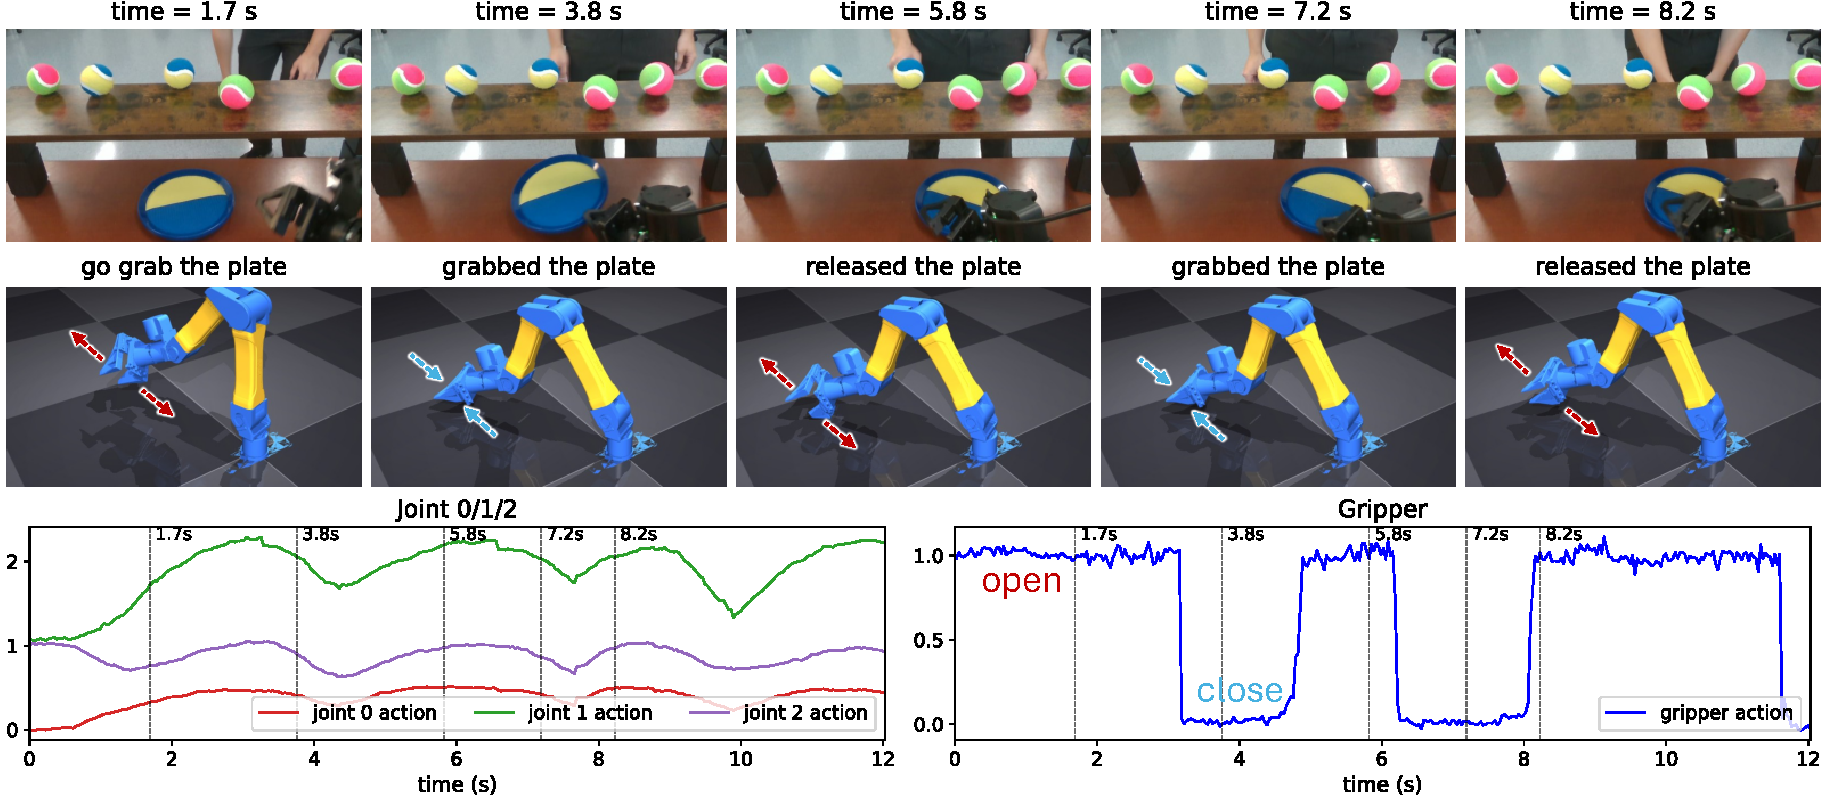
\includegraphics[width=\columnwidth]{2026-corl-unveil-template/figures/state_alias.pdf}
	\caption{\textbf{VLASH rollout on the untrimmed Flick Catch task.} The task is to grip the velcro plate and follow the human hand. VLASH's gripper hovers near the plate without committing to grasp or retract, because a single-frame observation cannot differentiate reaching for the plate from releasing it. RTC exhibits the same failure (see project page).}
	\label{fig:ambiguity}
\end{figure}

Because both baselines collapse to $0\%$ on the untrimmed task, a direct comparison there is uninformative. To enable a non-trivial comparison that isolates motion ambiguity from state aliasing, we manually trim the release-and-retract segment from every episode of the Flick Catch and Wine Pour training and evaluation data; the success rates on this trimmed version are reported in \cref{tab:success_rates}. The trimmed task still requires motion-aware perception (target tracking and timing) but removes the state-aliased segment.

To verify that \ours\ resolves state aliasing rather than merely benefiting from this trimming, we additionally train and evaluate every method on the original, untrimmed episodes. \cref{tab:state_alias} (in \cref{sec:diagnosis}) reports the resulting success rates: RTC and VLASH again fail every rollout, while \ours\ succeeds at $68\%$ on Flick Catch and $97.6$\% on Wine Pour. We attribute the gain to \TEMPOACT: the proprioceptive history distinguishes task phases that the current frame cannot, letting the policy commit to the correct action rather than hedging between reach-out and retract.

\section{Experimental Setup Details}
\label{app:setup}

\emph{Supplements \cref{sec:exp-setup}.}

\subsection{Hardware Platform}
All experiments are conducted on a bimanual workstation consisting of two I2RT YAM Ultra robot arms~\cite{i2rt_yam_ultra}, each with 7 degrees of freedom. The two arms are mounted and clamped to the table edge with their bases separated by 24 inches (61 cm). Both arms are placed on a rigid table measuring 6 ft × 29.5 in × 28 in (width × depth × height; 183 × 75 × 71 cm). Each arm is equipped with a parallel-jaw gripper.

 Visual observations are provided by three cameras: one fixed third-person camera positioned between the two arms and two wrist-mounted cameras. Each camera streams 224p at 30 Hz. Policies are executed at 30 Hz, if possible.

\subsection{Evaluation Protocol}

For the Drop Catch task, a single ball is released above the workspace from a height of 13–18 in (33–46 cm), measured from the table surface to the release point. The ball is tennis-ball sized and covered in a velcro-compatible material so that it adheres to the velcro plate that the gripper holds.

For the Flick Catch task, 5–6 balls are arranged on a shelf measuring 31.5 × 7.9 × 8.5 in (80 × 20 × 21.6 cm; width × depth × height), positioned near the table edge opposite to where the arms are clamped. These balls are identical to the one used in the Drop Catch task.

To ensure a fair evaluation, the human operator releasing the ball performs each trial with eyes closed while wearing headphones, preventing them from anticipating the robot's position and biasing the release point toward it.

\subsection{Training Details}

Each policy is trained on eight NVIDIA RTX PRO 6000 Blackwell GPUs. Training a single policy takes approximately 2 hours. More specifically, with an effective batch size of $128$ the per-iteration time is $0.49$s for VLASH, $0.46$s for RTC, and $0.50$s for \ours. RTC does not have an openly available codebase, so we reimplement it faithfully from its paper.


\section{Per-Task Failure Mode Breakdown}
\label{app:failure_breakdown}

\emph{Supplements \cref{sec:quant} and \figref{fig:failure_modes}.} To complement the Bottle Handover analysis in \cref{sec:quant}~(\figref{fig:failure_modes}), we apply the same protocol to Flick Catch and Drop Catch: we visually examine all $50$ rollouts per method on the trimmed task and assign each to a success or to one failure category. The categories differ across tasks because each task has different failure modes.

\begin{figure}[h]
	\centering
	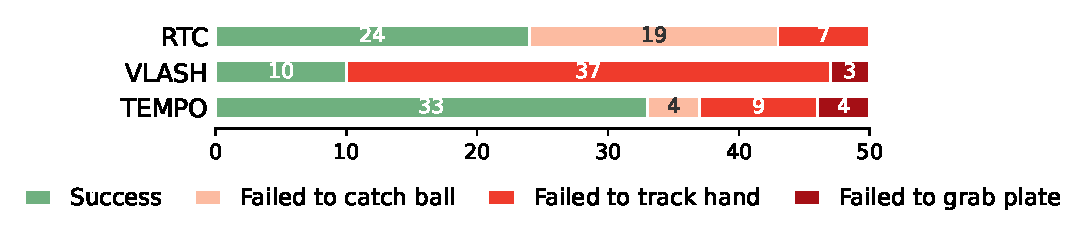
\includegraphics[width=\columnwidth]{2026-corl-unveil-template/figures/failure_modes_flick.pdf}
	\caption{\textbf{Failure-mode breakdown on Flick Catch.} Each of the $50$ rollouts is decomposed into success plus three failure modes corresponding to the three task stages (grab plate, track hand, catch ball). VLASH's failures concentrate in hand-tracking and RTC struggles most at tracking the ball's trajectory (see project page); \ours~cuts both failure modes.}
	\label{fig:flick_failure}
\end{figure}

\paragraph{Flick Catch (\figref{fig:flick_failure}).}
We assign each failed rollout to one of three failure modes corresponding to the three task stages: grabbing the plate, tracking the hand, or catching the flicked ball. VLASH's failures concentrate almost entirely in hand-tracking: in $37$ of $50$ trials the policy fails to follow the human hand and therefore never reaches the catching stage. RTC reacts to the hand but loses the flicked ball, with ball-catch failures accounting for $19$ trials, the dominant mode for RTC. \ours\ cuts VLASH's hand-tracking failures from $37$ to $9$ and RTC's ball-catch failures from $19$ to $4$; the residual failures are spread across all three stages rather than concentrated in any single one.

\begin{figure}[h]
	\centering
	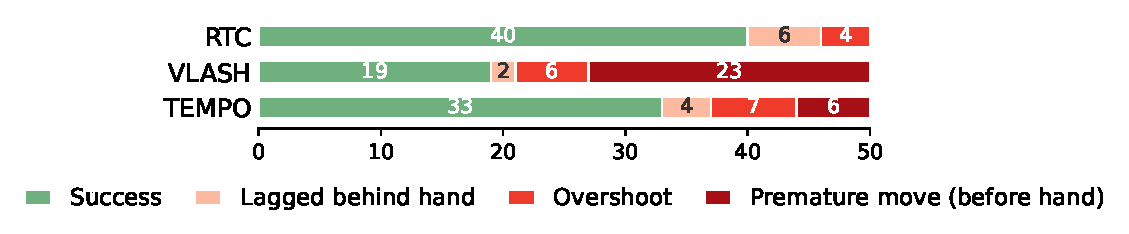
\includegraphics[width=\columnwidth]{2026-corl-unveil-template/figures/failure_modes_drop.pdf}
	\caption{\textbf{Failure-mode breakdown on Drop Catch.} RTC scores highest as Drop Catch is dominated by reactive timing rather than motion or state ambiguity. VLASH's dominant failure is premature movement before the human's hand begins to move; \ours\ cuts this failure by nearly $4\times$.}
	\label{fig:drop_failure}
\end{figure}

\paragraph{Drop Catch (\figref{fig:drop_failure}).}
Drop Catch is the timing-dominated task on which RTC scores highest~(\cref{tab:success_rates}); its only failures are a few overshoots ($4$) and lags ($6$). VLASH, despite also being asynchronous, exhibits a markedly different profile: it \emph{moves before the human's hand} in $23$ of $50$ trials, a near-majority failure that pulls its success rate down to $19$. \ours\ cuts this premature-move failure by nearly $4\times$ (from $23$ to $6$), with only a small change in overshoots ($6\to 7$). The premature-move reduction is consistent with the role of \TEMPOACT: the proprioceptive history records what the policy has already begun, so it does not re-initiate a move on every frame.


\begin{figure}[h]
	\centering    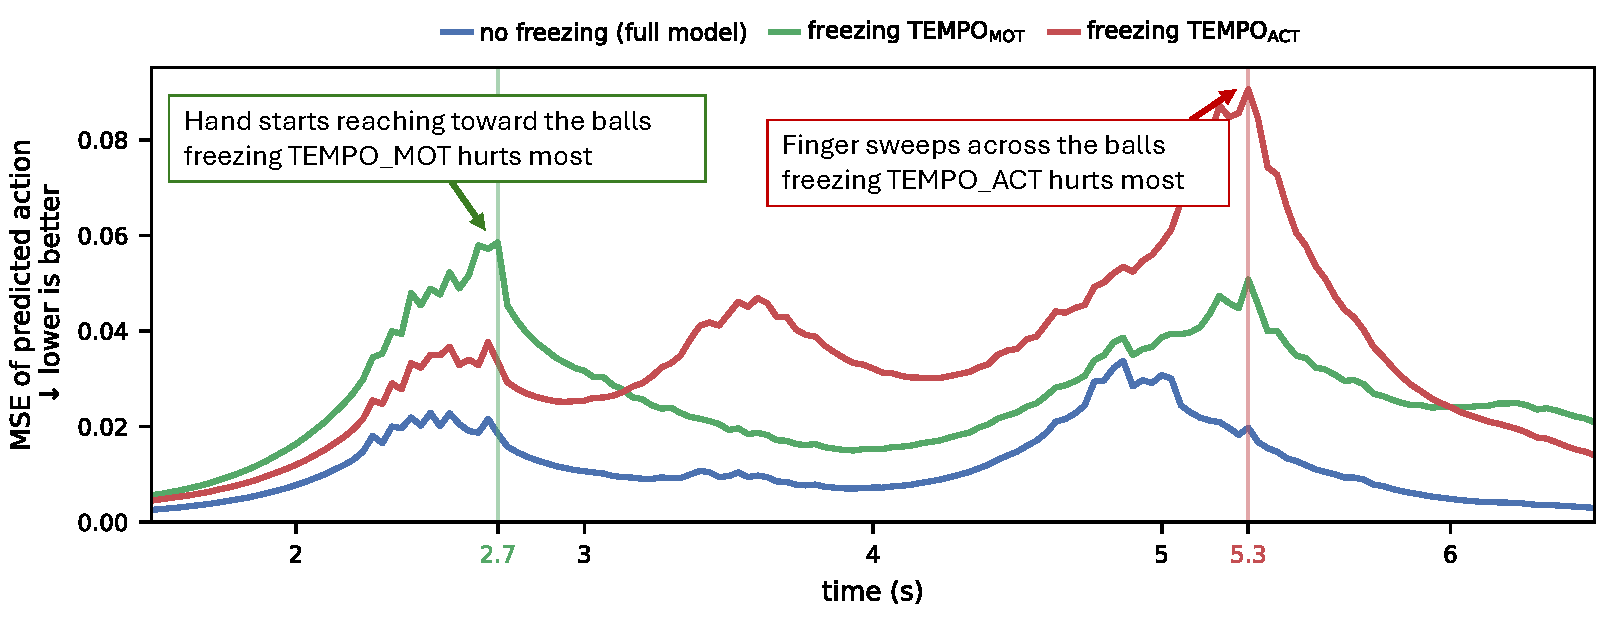
\includegraphics[width=0.9\columnwidth]{2026-corl-unveil-template/figures/ablation_mse.pdf}
	\vspace{-0.6em}
    \caption{\textbf{Both \TEMPOMOT\ and \TEMPOACT\ are necessary.} Per-frame action MSE for the full \ours\ model (blue) vs. the two single-signal ablations, evaluated on the Flick Catch task. Freezing \TEMPOMOT\ to its first-frame value (green) hurts most at $2.7$\,s, the beginning of the task where human hand starts to move. Freezing \TEMPOACT\ (red) hurts most at $5.3$\,s, the middle of the task where the finger sweeps horizontally across the balls before picking one and flicking it. Thus, each signal plays an important role at a different moment in the task.}
	\label{fig:attention_mse}
\end{figure}


\section{Input Ablation}
\label{app:input_ablation}




\emph{Supplements the modality-ablation analysis in \cref{sec:ablation}.}
To test whether \TEMPOMOT\ and \TEMPOACT\ are both necessary and contribute meaningfully to task performance, we run a per-frame ablation on a representative episode of the Flick Catch task (\figref{fig:attention_mse}). For each frame we ``remove'' each input modality by freezing \TEMPOMOT\ or \TEMPOACT\ to its first-frame value and measure the resulting predicted-action MSE; curves are EMA-smoothed for readability. Freezing either modality substantially degrades the policy's action prediction at different points in the episode. Freezing \TEMPOMOT\ hurts most at $2.7$\,s, the beginning of the task where large motions occur: MSE rises from $0.019$ to $0.059$ ($3.1\times$), while freezing \TEMPOACT\ costs only $0.033$. Freezing \TEMPOACT\ hurts most at $5.3$\,s, the middle of the task where the finger sweeps horizontally across the balls before picking one and flicking it, and there the pattern reverses: freezing \TEMPOACT\ hurts more than \TEMPOMOT\ ($0.091$ vs.\ $0.051$; full $0.020$). Each signal helps a different phase of the task.

\section{Motion Encoder Selection}
\label{app:motion_encoder}

\begin{figure}[h]
\centering

% --- Top row: per-task probing targets (image + label tightly coupled per panel) ---
\begin{minipage}[b]{0.235\columnwidth}
	\centering
	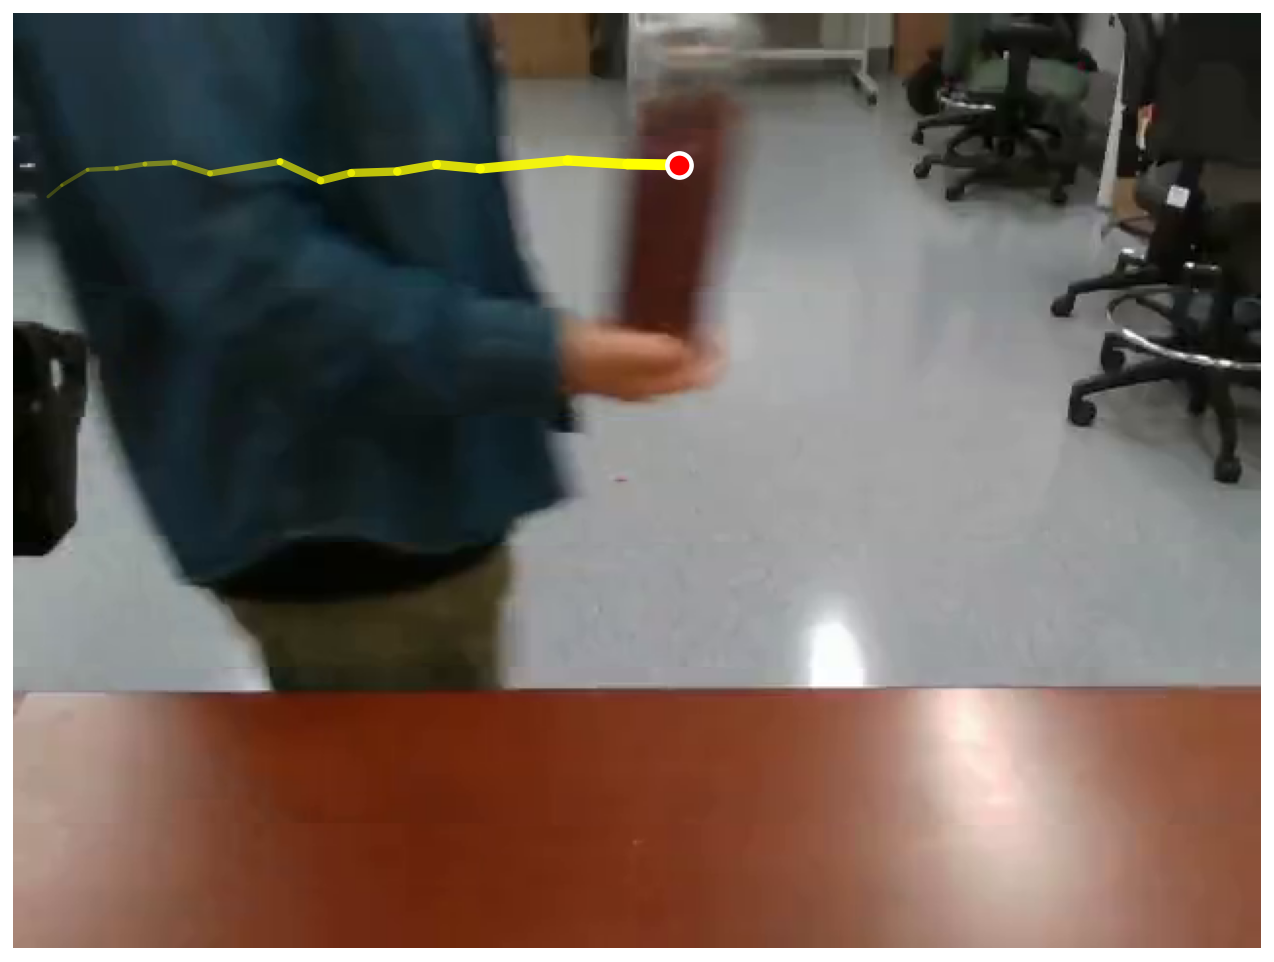
\includegraphics[width=\linewidth]{2026-corl-unveil-template/figures/velocity_handover.png}\\
	{\small Bottle Handover}
\end{minipage}\hfill
\begin{minipage}[b]{0.235\columnwidth}
	\centering
	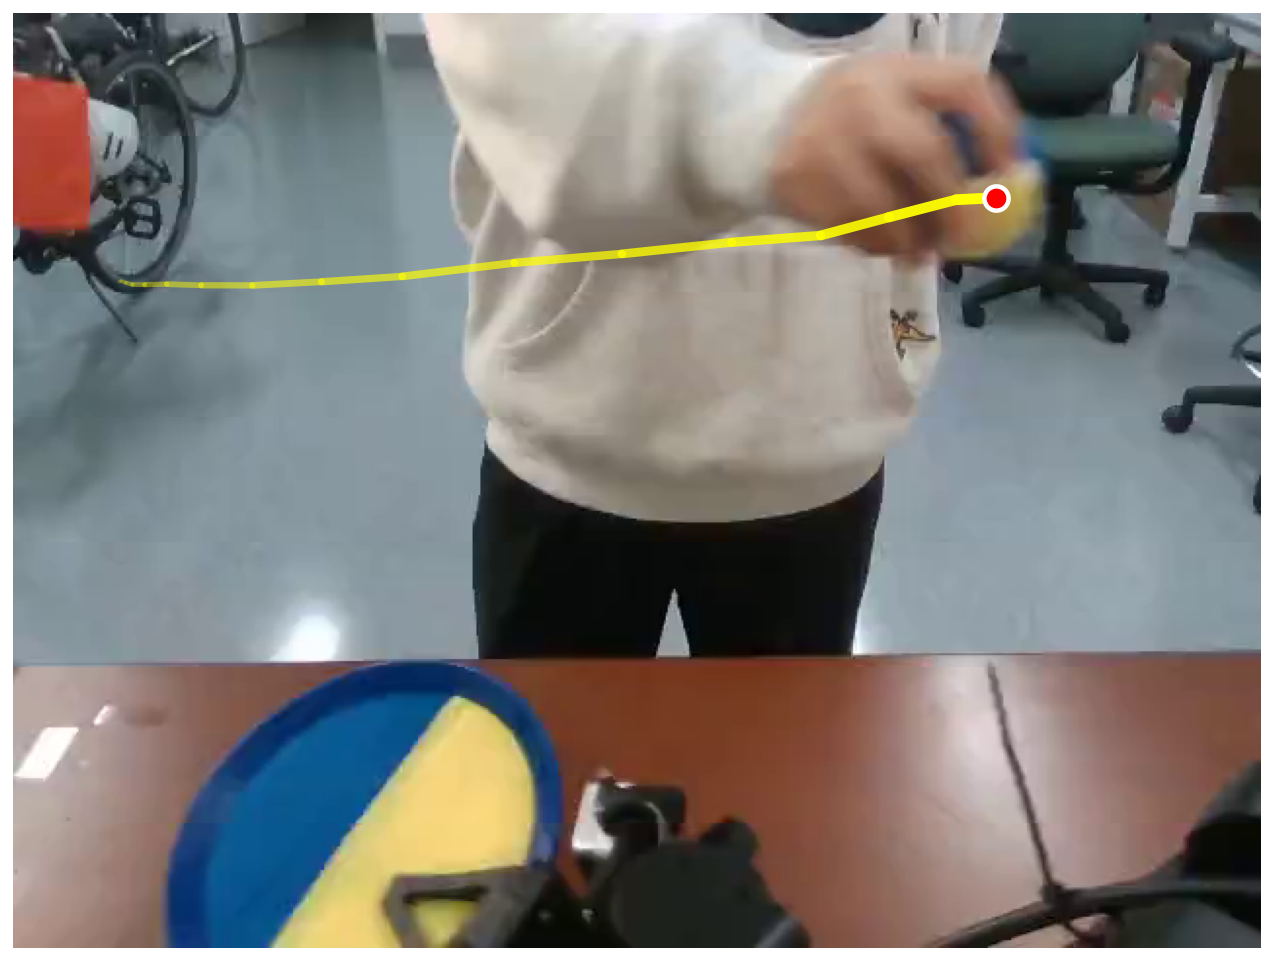
\includegraphics[width=\linewidth]{2026-corl-unveil-template/figures/velocity_drop.png}\\
	{\small Drop Catch}
\end{minipage}\hfill
\begin{minipage}[b]{0.235\columnwidth}
	\centering
	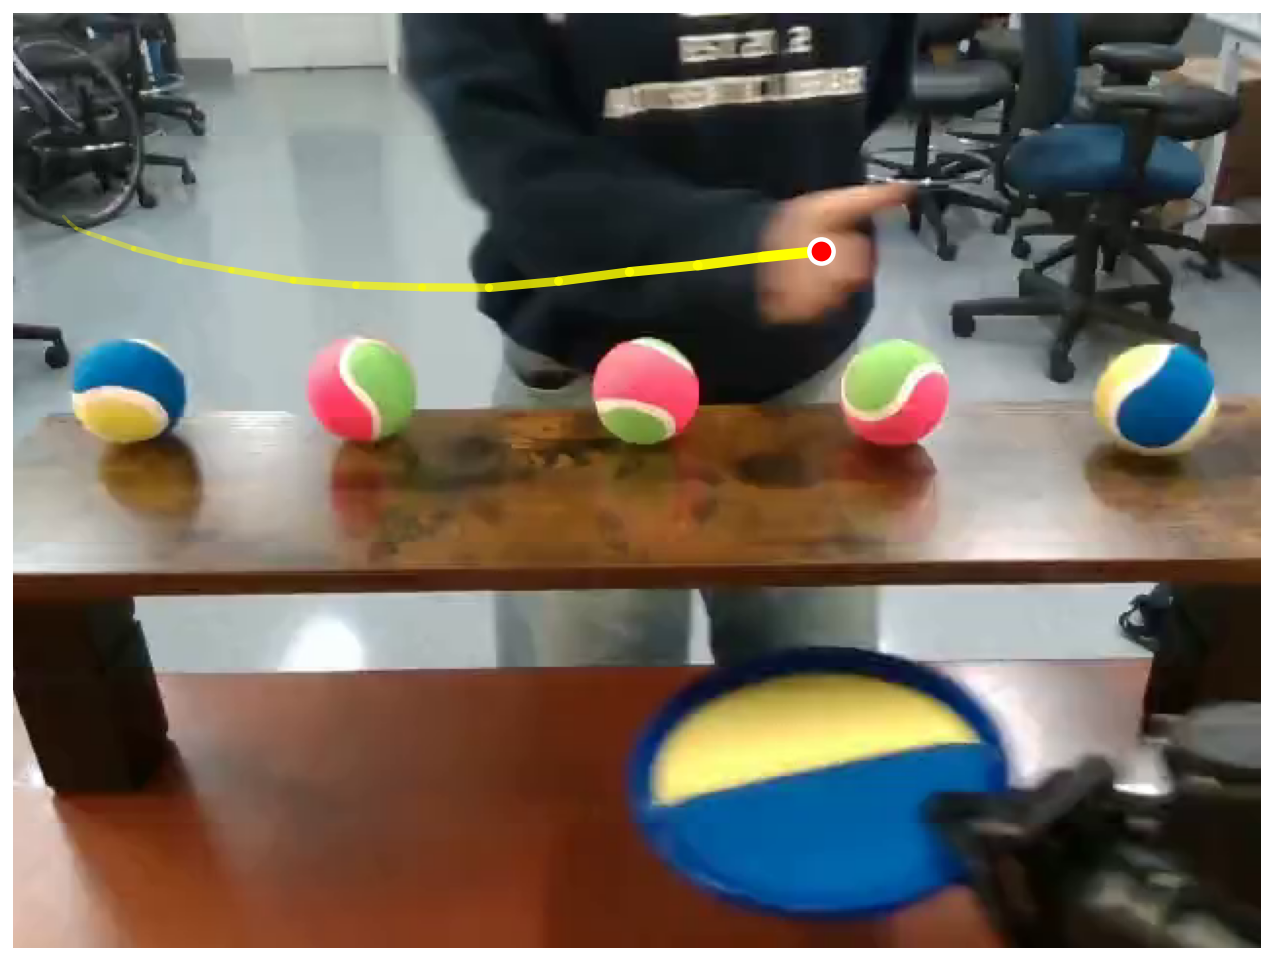
\includegraphics[width=\linewidth]{2026-corl-unveil-template/figures/velocity_flick.png}\\
	{\small Flick Catch}
\end{minipage}\hfill
\begin{minipage}[b]{0.235\columnwidth}
	\centering
	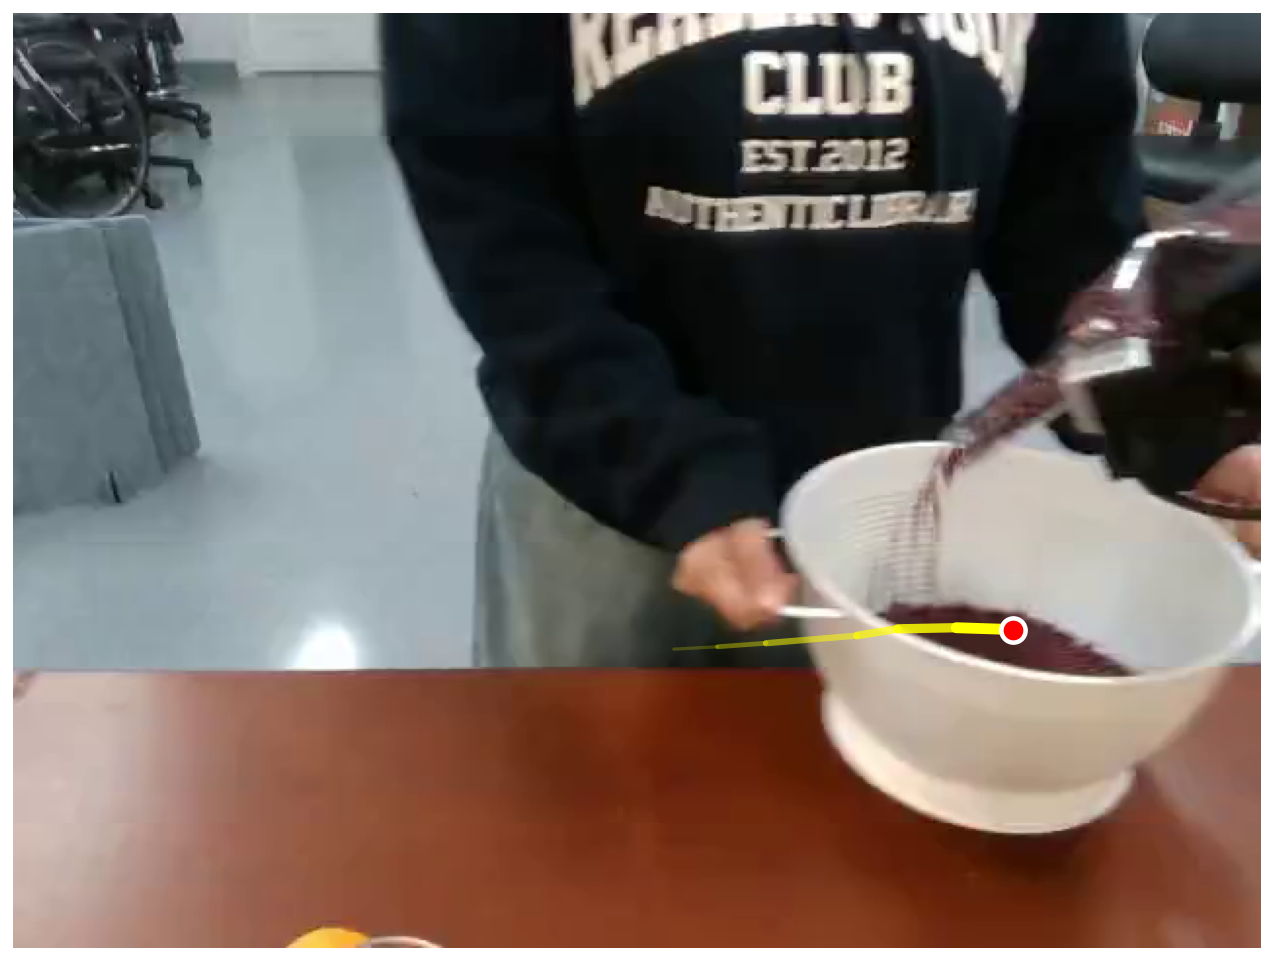
\includegraphics[width=\linewidth]{2026-corl-unveil-template/figures/velocity_pour.png}\\
	{\small Wine Pour}
\end{minipage}

\vspace{8pt}

% --- Bottom: probe results ---
\small
\begin{tabular}{lccccc}
\toprule
\textbf{Initialization for \TEMPOMOT} & \textbf{Bottle Handover} & \textbf{Drop Catch} & \textbf{Flick Catch} & \textbf{Wine Pour} & \textbf{Average} \\
\midrule
% Random                                & -0.01 & 0.00 & 0.00 & 0.00 & 0.00 \\
Object Position                          & 0.24  & 0.03 & 0.03 & 0.02 & 0.08 \\
VideoLaVIT~\cite{videolavit}             & 0.45  & 0.25 & 0.28 & 0.36 & 0.34 \\
Reducio~\cite{reducio}                   & 0.50  & 0.36 & 0.38 & 0.32 & 0.39 \\
SAM~2~\cite{sam2}                        & 0.58  & 0.37 & 0.50 & 0.39 & 0.46 \\
VidTwin~\cite{vidtwin}                   & 0.59  & 0.44 & 0.43 & 0.45 & 0.48 \\
\bottomrule
\end{tabular}

\caption{\textbf{Linear probe of candidate initializations for \TEMPOMOT.} \emph{Top:} one example frame per task showing the object of interest (red dot) and its recent trajectory (yellow line); the pixel-space velocity of this object is the regression target the linear probe must predict. \emph{Bottom:} per-task velocity $R^2$ for each candidate initialization, along with the average. Higher is better; the raw object-position baseline ($R^2=0.08$ on average) cannot recover velocity from a single position, while every learned motion encoder does so substantially better.}
\label{fig:ball_velocity_probe}
\end{figure}


\emph{Supplements the motion-encoder definition in \cref{sec:method} (the $\phi$ in \TEMPOMOT).}
\ours\ is agnostic to the choice of motion encoder; here we justify ours. Reusing the per-frame object-velocity annotation from our motion probe (\secref{sec:analysis}; the per-task probing target is visualized at the top of \figref{fig:ball_velocity_probe}), we fit a \emph{linear} probe from each candidate motion latent to the object's velocity: if the latent captures the object's motion, a linear readout should recover the velocity with high $R^2$. Every learned encoder decodes velocity far above the raw object position (avg.\ $R^2 = 0.08$), confirming that object motion is genuinely present in the latent and that a single position, like a single frame, does not by itself encode meaningful information to infer object motion. SAM~2 and VidTwin score highest; we adopt SAM~2.1-Tiny because it pairs near-top motion correlation with the streaming speed required for real-time deployment (\cref{tab:latency_comparison}).
